\renewcommand{\thesubfigure}{\alph{subfigure}}
\renewcommand{\figurename}{Figure}
\renewcommand{\tablename}{Table}
\setcounter{figure}{0}
\setcounter{table}{0}

\chapter*{Synopsis}
\addcontentsline{toc}{chapter}{Synopsis} 

\begin{center}
    General thesis summary
\end{center}
\begin{figure}
	\centering
	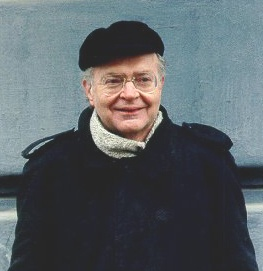
\includegraphics[width=0.4\linewidth]{images/knuth}
	\caption{Knuth}
	%\label{fig:my_label2}
\end{figure}
\begin{table}
	\centering
	\captionsetup{justification=centering} % выравнивание подписи по-центру
	\caption{Basic SI quantities}%\label{tab:unit:base}
	\begin{tabular}{llc}
		\toprule
		Name 	& 	Command 	& 	Symbol         \\
		\midrule
		Ampere     & \verb|\ampere| & \si{\ampere}   \\
		Candela   & \verb|\candela| & \si{\candela}  \\
		\bottomrule
	\end{tabular}
\end{table}

\paragraph*{Relevance of the chosen topic.}
\paragraph*{Goal.}
\paragraph*{Objectives.}
\paragraph*{Research methods.}
\paragraph*{Assertions that are presented for defense.}
\paragraph*{The novelty of research.}
\paragraph*{The scientific and technical objective.}
\paragraph*{The research object.}
\paragraph*{The research subject.}
\paragraph*{The theoretical significance.}
\paragraph*{The practical significance.}
\paragraph*{The accuracy of the obtained results.}

\paragraph*{Implementation of research results.}
\paragraph*{Approbation of research results.}
The main results of the thesis were presented at the following conferences:
\begin{enumerate}
	\item \textcolor{blue}{The 22nd IFAC World Congress}, Yokohama, Japan.  July 9--14, 2023.
	\item \textcolor{blue}{The 63rd IEEE Conference on Decision and Control (CDC-2024)}, Milan, Italy. December 16--19, 2024.
	\item \textcolor{blue}{XIV All-Russian Conference on Management Issues (VSPU-2024)}, IPU RAS Moscow, Russia. June 17--20, 2024.
	%XIV Всероссийское совещание по проблемам управления, Россия, Москва, ИПУ РАН, 17-20 июня 2024
\end{enumerate}
\paragraph*{Personal contribution of the author.}
\paragraph*{Thesis structure and number of pages.}

\newpage
\section*{Main contents of the work}

In Chapter~\ref{ch:ch1}...

\section*{Publications relevant to this thesis}
%Key results of research are described in nine publications. Four of them are published in journals recommended by the Higher Attestation Commission and one is published in a journal indexed by Scopus. One certificate of state registration of a computer program has also been obtained.\\
Key results of research are described in \theAllPapers~publications. Among them \theScopusPapers~are published in a journal indexed by Scopus and Web of Science. 
%and 0 published in journals recommended by the Higher Attestation Commission (VAK) 
%and 1 is published in other sources.

Publications in international journals indexed by Scopus and Web of Science:
\insertpapperScopus
%Publications indexed in Russian journal included in the List of the Higher Attestation Commission: 

Publications in other journals:
\insertpapperOther